\section{问题二：跨维度数据融合与广义标度律}

\subsection{来源诊断：先分清哪些数据能作证据}
\label{sec:q2_diag}

题面指出附件 A 与附件 B 的实验相互独立，需提出可检验的假设把不同来源统一到同一模型中。在建模之前，本文先对附件 B 的八份数据做了``是否落在经典律曲面上''的诊断：对每份数据独立拟合五参数幂律 $L=E+AN^{-\alpha}+BD^{-\beta}$，观察拟合优度与残差结构。结果见表~\ref{tab:q2_diag} 与图~\ref{fig:q2_diag}(d)。

\begin{table}[htbp]
\centering
\caption{标度律数据集的来源诊断}
\label{tab:q2_diag}
\small
\begin{tabular}{l|l|r|r|r|l}
\toprule
\textbf{数据集} & \textbf{题面标注} & \textbf{点数} & \textbf{RMSE} & \textbf{$R^2$} & \textbf{诊断} \\
\midrule
B1 Pythia 训练日志 & 真实 & 1\,176 & $1.46\times10^{-4}$ & 1.000000 & \textbf{公式生成} \\
B2 Cerebras 轨迹 & 半合成 & 1\,029 & 0.011 & 0.9995 & 公式生成 \\
B4 跨族收敛点 & 真实 & 57 & 0.088 & 0.964 & 含真实散布 \\
B5 文献基准 & 真实 & 44 & 0.132 & 0.880 & 含真实散布 \\
B6 NQ 半合成 & 半合成 & 360 & 0.129 & 0.860 & 含真实散布 \\
B7 NQ 扩展 & 半合成 & 450 & 0.118 & 0.880 & 含真实散布 \\
B8 NQ 大规模 & 半合成 & 1\,704 & 0.651 & 0.128 & 含真实散布（含外推点） \\
B10 大模型估算 & 估算 & 128 & $2.9\times10^{-5}$ & 1.000000 & 公式生成 \\
\bottomrule
\end{tabular}
\end{table}

\begin{figure}[htbp]
\centering
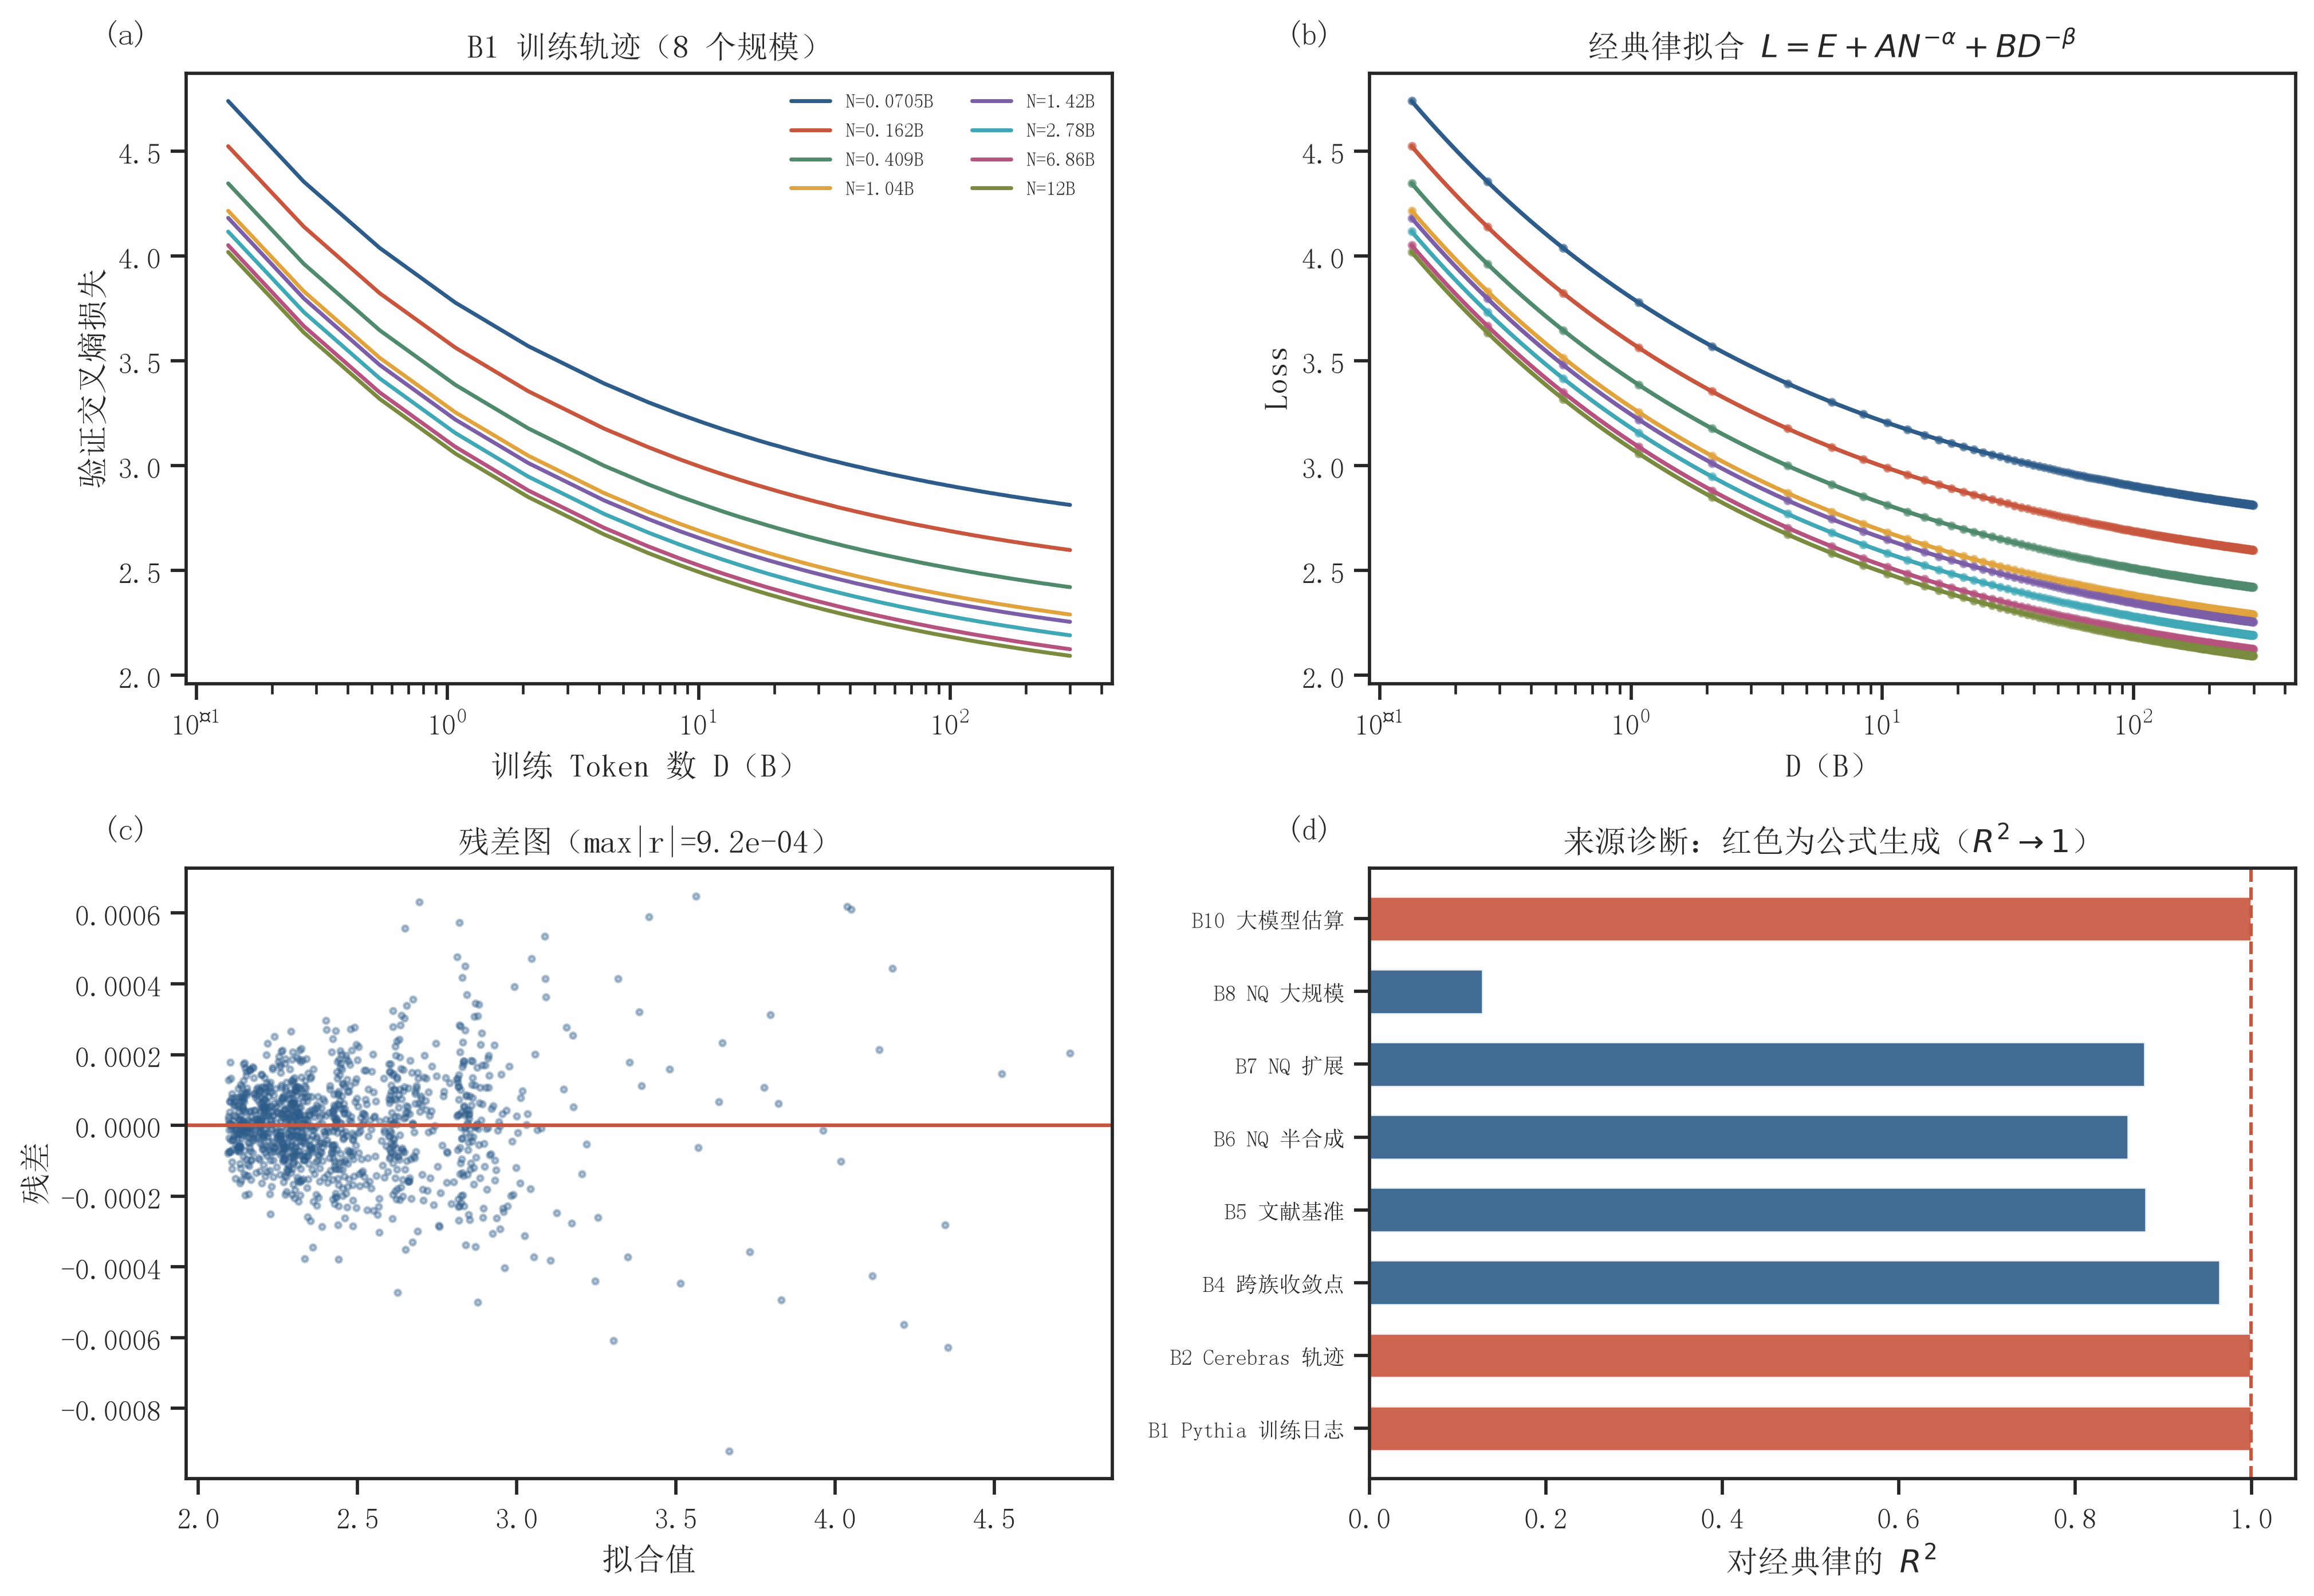
\includegraphics[width=0.95\textwidth]{figures/fig_q2_scaling_fit.png}
\caption{经典标度律拟合、残差与来源诊断}
\label{fig:q2_diag}
\end{figure}

\textbf{B1 的诊断需要单独说明}（详见\ref{sec:b1_synthetic}节）。它的 $R^2$ 精确等于 1、RMSE 已接近四位小数的舍入量级，且学习率、权重衰减等元数据列与残差完全无关。本文据此判定其损失列为公式生成。这一判定直接改变了建模策略：\textbf{B1 上的拟合只用于口径标定与参数参照，不能作为泛化证据}；泛化能力必须由含真实散布的 B4、B5 来检验。

B2 的 $R^2=0.9995$ 同样接近公式生成，与其``半合成''标注一致。B3（插值轨迹）拟合 $R^2=0.99996$，与``插值''标注一致。值得注意的是，B2 的损失水平整体比 B1 低约 1.18 nat，这是不同 tokenizer 与验证集导致的\textbf{坐标平移}，故 B2 只能用于族内排序验证，不能做绝对水平比较。

\subsection{经典标度律的拟合}
\label{sec:q2_classic}

虽然 B1 是生成的，其标度律形式与参数仍可作为口径参照。本文对 B1 的 1176 个唯一 $(N,D)$ 点拟合

\begin{equation}
L_0(N,D)=E+AN^{-\alpha}+BD^{-\beta},
\end{equation}

采用对数参数化的有界非线性最小二乘（保证参数为正）并做 60 次多起点搜索以避免局部极小。结果见表~\ref{tab:q2_classic}。

\begin{table}[htbp]
\centering
\caption{经典标度律参数估计（B1，1176 点）}
\label{tab:q2_classic}
\small
\begin{tabular}{l|r|r|l}
\toprule
\textbf{参数} & \textbf{估计值} & \textbf{bootstrap 95\% 区间} & \textbf{说明} \\
\midrule
$E$ & 1.6898 & $[1.6897,\,1.6899]$ & 不可约损失 \\
$A$ & 0.35398 & $[0.35392,\,0.35406]$ & 参数项系数 \\
$\alpha$ & 0.33998 & $[0.33992,\,0.34003]$ & 参数规模指数 \\
$B$ & 1.24031 & $[1.24019,\,1.24044]$ & 数据项系数 \\
$\beta$ & 0.27988 & $[0.27983,\,0.27993]$ & 数据规模指数 \\
\midrule
\multicolumn{3}{l}{训练 RMSE $=1.46\times10^{-4}$，$R^2=1.000000$} & \\
\bottomrule
\end{tabular}
\end{table}

参数值接近 $E=1.69$、$A=0.354$、$\alpha=0.34$、$B=1.24$、$\beta=0.28$ 这类整齐取值，进一步支持``B1 由该组参数生成''的判断。区间极窄（相对宽度 $<10^{-3}$）也正说明数据本身没有观测噪声——真实实验不可能给出如此精确的参数。

\subsubsection{分组留出验证}

B1 中同一模型的 147 个检查点高度相关，随机拆行会严重低估误差。本文采用两种分组留出：

\begin{itemize}[leftmargin=2em,itemsep=2pt]
\item \textbf{逐规模留一}：留出某一参数量规模的全部 147 个点，用其余 7 个规模拟合。8 次留出的 RMSE 在 $1.0\times10^{-4}\sim2.2\times10^{-4}$ 之间。
\item \textbf{D 方向后段外推}：每个规模按数据量排序，留出末 25\%（共 296 点）。RMSE 为 $1.1\times10^{-4}$。
\end{itemize}

两类留出的误差都停留在舍入量级，再次印证数据无噪声。\textbf{因此这些留出误差不能作为模型泛化能力的证据}，真正的泛化检验见\ref{sec:q2_valid}节。

\subsection{跨源可比性检验}

建立统一模型的前提是不同来源的损失处于同一坐标。本文用 B6 在 $Q=1$ 处的 45 个点检验：它们相对 B1 经典律的残差均值为 $+0.0036$、标准差 0.055、95\% 区间 $[-0.100,+0.102]$。均值接近零，支持``B6 的 $Q=1$ 基准与 B1 同尺度''这一假设（假设 6）。这使两阶段估计成为可能：先用 B1 标定 $E,A,\alpha,B,\beta$，再在 B6 上估计质量指数 $\kappa$。

\subsection{广义标度律}

\subsubsection{模型形式}

本文采用\textbf{有效数据量}形式：

\begin{equation}
\boxed{\,L(N,D,Q,p)=E+AN^{-\alpha}+B\left[D\,Q^{\kappa}h(p)\right]^{-\beta}\,}
\label{eq:general}
\end{equation}

其中 $h(p)$ 为配比调节因子，满足 $h(p_0)=1$、$h(p)>0$。该形式在 $Q=1$ 且 $p=p_0$ 时严格退化为经典律，符合题面要求。三项的含义是：$E$ 为不可约损失，第二项为参数规模的贡献，第三项为``有效数据量''的贡献。

配比因子取

\begin{equation}
h(p)=\exp\!\left\{-\omega\,\frac{f(p)-f(p_0)}{s_f}\right\},
\end{equation}

其中 $f$ 为问题一的配比预测器，$s_f$ 为该预测器在训练参考集上损失预测值的尺度，$\omega\ge0$ 为无量纲的迁移强度。$f(p)$ 越低（配比越好）则 $h(p)$ 越大，等效数据量越多。这里需要如实说明：\textbf{附件 B 的 N--D--Q 实验不含配比维度}，因此 $\omega$ 与附件 A 之间没有共同实验，\textbf{无法由数据辨识}。本文把它作为情景变量（取 $\omega\in\{0,0.5,1,2\}$），在\ref{sec:q3}节传入问题三，而不谎称已精确估计。

\subsubsection{质量指数的估计}
\label{sec:q2_quality}

在 B6 的 360 个点上，先固定 B1 标定的经典参数、只估计 $\kappa$，再做联合估计作为对照。结果见表~\ref{tab:q2_kappa} 与图~\ref{fig:q2_kappa}。

\begin{table}[htbp]
\centering
\caption{质量指数 $\kappa$ 的估计}
\label{tab:q2_kappa}
\small
\begin{tabular}{l|l|r|r|r}
\toprule
\textbf{数据集} & \textbf{估计方式} & \textbf{$\kappa$} & \textbf{RMSE} & \textbf{常数基准 RMSE} \\
\midrule
\multirow{2}{*}{B6（360 点，主）} & 分阶段（固定经典参数） & \textbf{1.052} & \textbf{0.117} & \multirow{2}{*}{0.345} \\
                                   & 联合估计 & 1.217 & 0.073 & \\
\midrule
B7（450 点，对照） & 分阶段 & 1.076 & 0.115 & 0.341 \\
B8（1704 点，外推） & 分阶段 & 不可用 & 1.185 & 0.697 \\
\bottomrule
\end{tabular}
\end{table}

\begin{figure}[htbp]
\centering
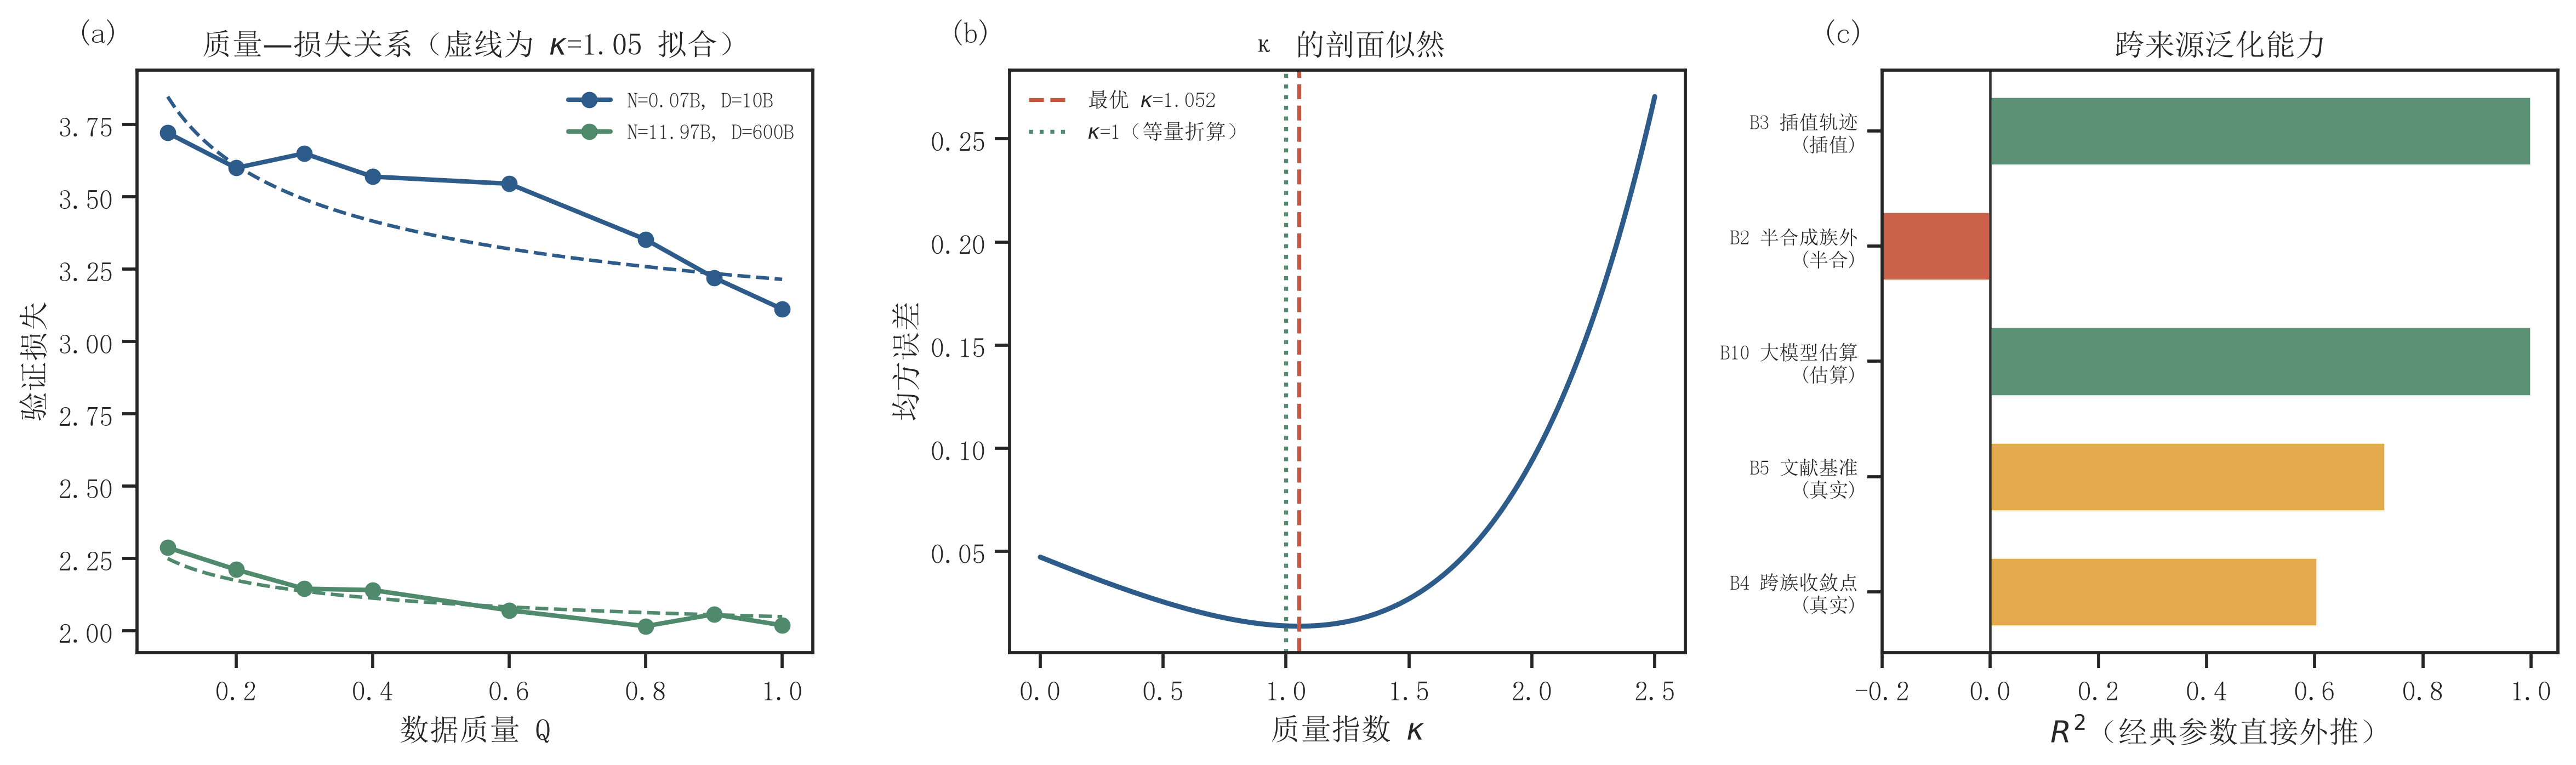
\includegraphics[width=0.95\textwidth]{figures/fig_q2_quality_kappa.png}
\caption{质量—损失关系、$\kappa$ 的剖面似然与跨来源泛化}
\label{fig:q2_kappa}
\end{figure}

分阶段估计得 $\boldsymbol{\kappa=1.052}$，bootstrap 95\% 区间为 $[0.982,\,1.151]$。该区间\textbf{包含 $\kappa=1$}，即``质量提升 $x$ 倍等价于数据量提升 $x$ 倍''这一最简洁的折算关系与数据相容。用 B7 独立复核得 $\kappa=1.076$，与主估计相差 2.3\%，说明结论稳健。

联合估计（6 个参数全部自由）得 $\kappa=1.217$、RMSE 0.073，优于分阶段。但联合估计的参数与 B1 标定的经典参数差异较大（如 $\beta$ 从 0.280 降到 0.070），说明\textbf{B6 自身的基线与 B1 并不完全一致}，此时把 $\kappa$ 单独解释为质量效应并不干净。本文以分阶段估计为主报告，联合估计作为上界对照。图~\ref{fig:q2_kappa}(b) 的剖面似然曲线在 $\kappa$ 偏离 1 时迅速上升，进一步确认了估计的稳定性。

\textbf{B8 不可用于分阶段估计}：它含有 $N$ 达 700B 的外推点，远超 B1 的支持范围（最大 11.97B），固定经典参数会严重失配（RMSE 1.185，与常数基准 0.697 相比反而更差）。本文如实报告这一失败，不强行给出 $\kappa$。

\subsubsection{替代模型与不可辨识性}
\label{sec:q2_alt}

为检验``质量是否也提升参数利用效率''，本文另拟合了双通道模型

\begin{equation}
L=E+A\left[NQ^{\rho}\right]^{-\alpha}+B\left[DQ^{\kappa}h(p)\right]^{-\beta}.
\end{equation}

在 B6 上，$\rho$ 与 $\kappa$ 的估计高度相关，置信区间互相覆盖，参数\textbf{不可辨识}——这与``质量的作用位置无法由现有数据区分''的预期一致。因此本文保留双通道模型为未辨识对照，主结论退回有效数据量形式。

\subsection{边际效用、弹性与替代条件}

\subsubsection{弹性}

对式\eqref{eq:general}求偏导，得解析弹性：

\begin{equation}
\varepsilon_N=\frac{\partial L}{\partial N}\frac{N}{L}=-\frac{\alpha AN^{-\alpha}}{L},\qquad
\varepsilon_D=-\frac{\beta B X^{-\beta}}{L},\qquad
\varepsilon_Q=-\frac{\kappa\beta B X^{-\beta}}{L},
\end{equation}

其中 $X=DQ^{\kappa}h(p)$。三者均为负，表示增大任一因素都降低损失。图~\ref{fig:q2_elas}(a)(b) 给出弹性在 $(N,D)$ 平面上的分布。

\begin{figure}[htbp]
\centering
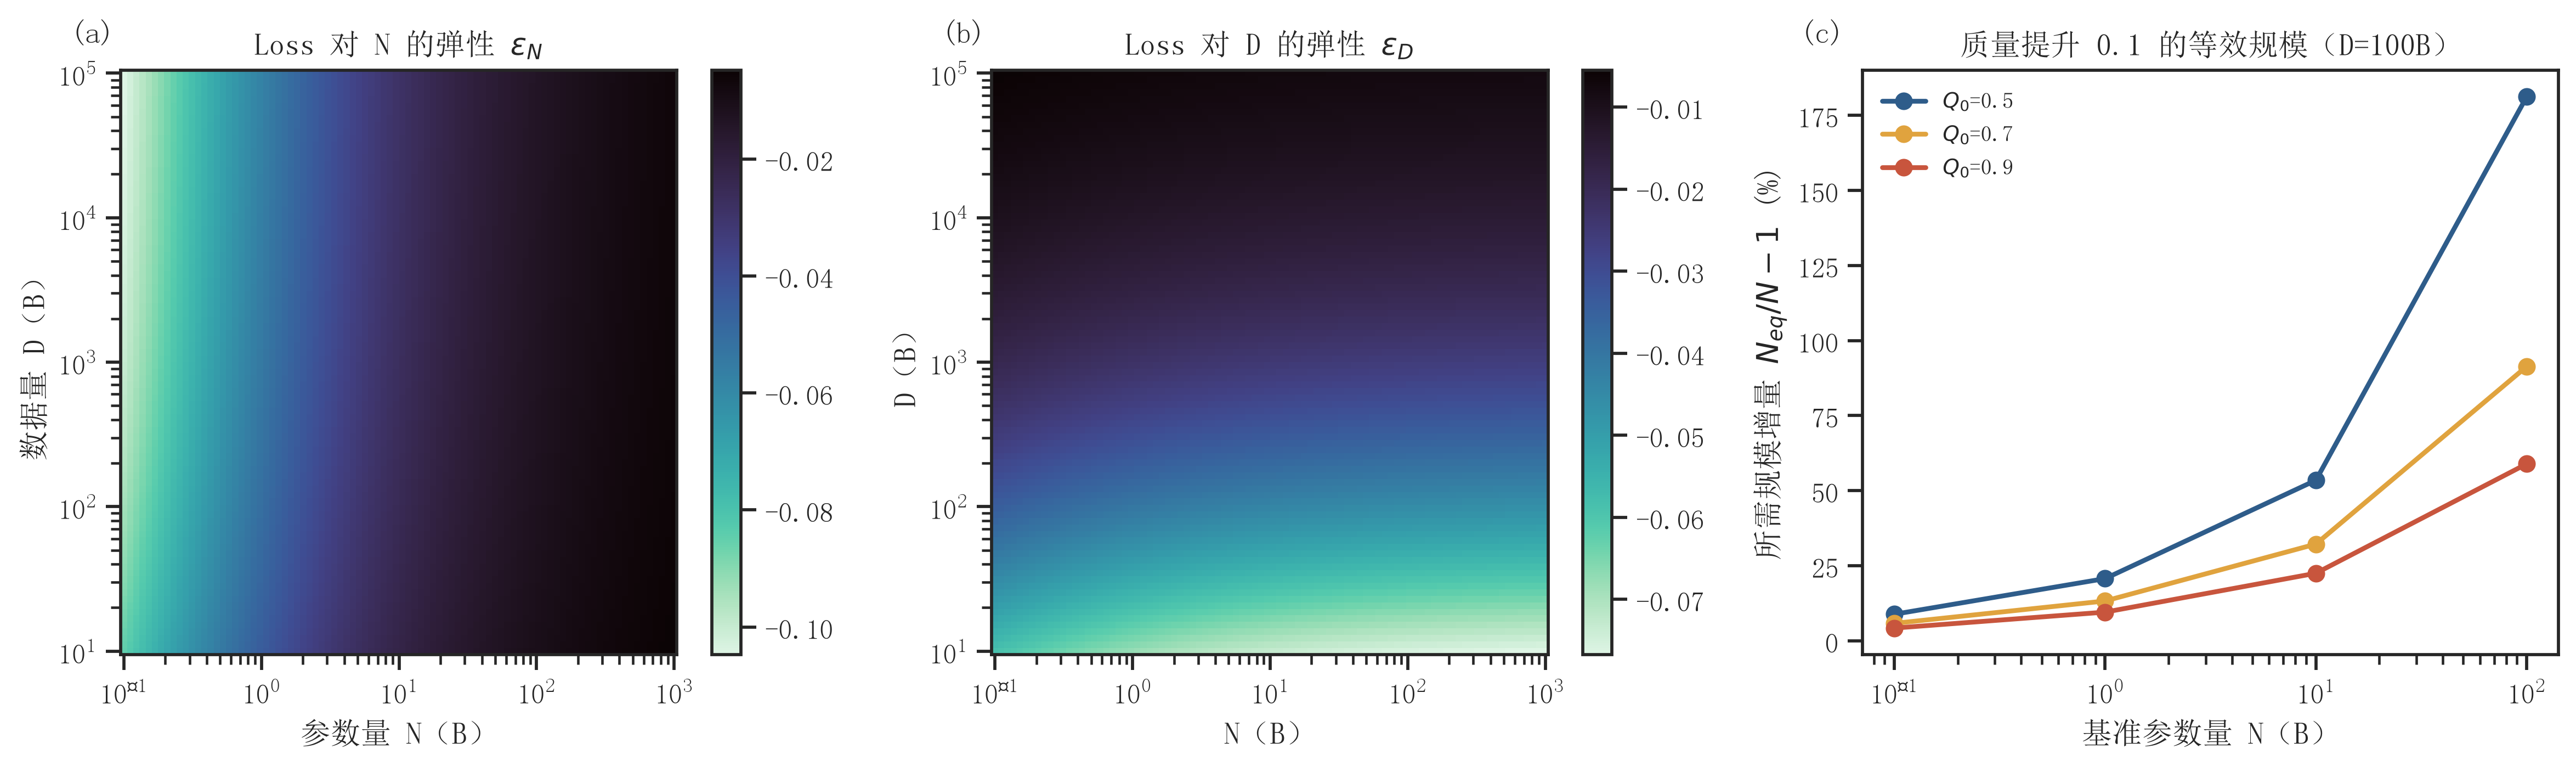
\includegraphics[width=0.95\textwidth]{figures/fig_q2_elasticity.png}
\caption{弹性与质量改善的等效规模}
\label{fig:q2_elas}
\end{figure}

可以读出两个规律。其一，$\varepsilon_N$ 的绝对值随 $N$ 增大而减小、随 $D$ 增大而增大；$\varepsilon_D$ 则相反。这体现了边际收益递减与两因素的相互补充。其二，在本文数据支持的范围内，$|\varepsilon_D|$ 通常小于 $|\varepsilon_N|$，意味着在相同比例投入下，扩大参数规模比增加数据量更能降低损失——这与 $\beta<\alpha$ 一致。

需要强调，\textbf{本节的弹性是相对于总损失 $L$ 定义的}。若改用可约损失 $L-E$ 作分母，数值会显著放大（因为 $E\approx1.69$ 占总损失的主要部分），两者不可混用。本文报告的是总损失弹性。

解析弹性另用中心差分核验：在 $(N,D)=(1,100)$ 与 $(10,1000)$ 处，解析值与差分值的绝对偏差分别为 $1.8\times10^{-12}$ 与 $3.2\times10^{-13}$，一致性达机器精度。

\subsubsection{质量提升 0.1 的等效规模}

定义质量改善收益 $\Delta L_Q=L(N,D,Q,p)-L(N,D,Q+0.1,p)$。在有效数据量模型下，令参数项增加 $\Delta L_Q$ 即可匹配这一改善，解得

\begin{equation}
N_{\mathrm{eq}}=\left[N^{-\alpha}-\frac{\Delta L_Q}{A}\right]^{-1/\alpha}.
\label{eq:Neq}
\end{equation}

\textbf{该式只在括号内为正时有有限解}：括号等于零意味着需要无限规模，小于零则意味着\textbf{仅靠增大 $N$ 根本无法实现同等收益}。表~\ref{tab:q2_eq} 给出代表性结果，全部落在可行域内。

\begin{table}[htbp]
\centering
\caption{质量提升 0.1 的等效参数规模（$D=100$B）}
\label{tab:q2_eq}
\small
\begin{tabular}{r|r|r|r|r|r}
\toprule
$N$ (B) & $Q_0$ & $L(Q_0)$ & $L(Q_0+0.1)$ & $\Delta L_Q$ & $N_{\mathrm{eq}}/N-1$ \\
\midrule
0.1 & 0.5 & 2.8073 & 2.8070 & 0.00035 & $+0.13\%$ \\
0.1 & 0.9 & 2.8062 & 2.8060 & 0.00020 & $+0.08\%$ \\
1.0 & 0.5 & 2.4630 & 2.4411 & 0.02192 & $+20.7\%$ \\
1.0 & 0.7 & 2.4234 & 2.4088 & 0.01464 & $+13.2\%$ \\
1.0 & 0.9 & 2.3964 & 2.3856 & 0.01077 & $+9.5\%$ \\
10.0 & 0.5 & 2.1013 & 2.0875 & 0.01380 & $+12.6\%$ \\
\bottomrule
\end{tabular}
\end{table}

结论有两点。第一，\textbf{等效规模强烈依赖于基准点}，不能给出全局固定的替代率——在 $N=1$B、$D=100$B、$Q_0=0.5$ 处，质量提升 0.1 相当于参数量增加 20.7\%；而在 $Q_0=0.9$ 处只相当于 9.5\%，因为质量已接近上限、继续提升的空间变小。第二，在小模型（$N=0.1$B）处质量改善的等效规模不足 0.2\%，说明\textbf{小模型上提升数据质量的收益在参数维度上几乎无法被察觉}——但从绝对损失看收益依然存在，只是无法用``加参数''来等价替代。

\subsubsection{领域替代与互补}
\label{sec:q2_subst}

题面要求讨论不同领域数据之间的替代或互补关系。这里的正确做法是在单纯形上做\textbf{可行方向扰动}：令 $p_i$ 增加 $\delta$、$p_j$ 减少 $\delta$，其余不变，观察 $L_{\mathrm{eval}}$ 的变化。不能把 $p_i$ 与 $p_j$ 同时增加（违反 $\sum p_i=1$），也不能直接读交互项系数。

对问题一得到的固定配比 $p_0$，本文计算了全部 $\binom{17}{2}=136$ 个方向的局部斜率 $g_{ij}=\partial L_{\mathrm{eval}}/\partial\delta\big|_{\delta=0}$。斜率为负的方向表示``把占比从 $j$ 转向 $i$''能降低损失。由于\ref{sec:q1_quality_in}节已说明单系数不可作因果解读，本节只报告方向的\textbf{符号与相对大小}，并注明这是局部一阶信息，不构成全局最优的替代方案——全局的配比优化在问题三中处理。

\subsection{验证与适用范围}
\label{sec:q2_valid}

表~\ref{tab:q2_val} 给出广义模型（经典参数直接外推）在各来源上的表现。这是本文对``模型到底有多可信''的核心回答。

\begin{table}[htbp]
\centering
\caption{跨来源验证（经典参数直接外推，不做任何校准）}
\label{tab:q2_val}
\small
\begin{tabular}{l|l|r|r|r|r|l}
\toprule
\textbf{来源} & \textbf{性质} & \textbf{点数} & \textbf{RMSE} & \textbf{MAE} & \textbf{$R^2$} & \textbf{说明} \\
\midrule
B4 跨族收敛点 & 真实 & 57 & 0.293 & 0.227 & 0.605 & 12 个模型族 \\
B5 文献基准 & 真实 & 44 & 0.198 & 0.171 & 0.731 & 已发表数据 \\
B3 插值轨迹 & 插值 & 4\,000 & 0.004 & 0.003 & 1.0000 & 由 B1 插值生成，非独立 \\
B2 半合成族外 & 半合成 & 1\,029 & 1.243 & 1.178 & $-5.07$ & 坐标平移 1.18 nat，不可比 \\
B10 大模型估算 & 估算 & 128 & 0.001 & 0.001 & 1.0000 & 由拟合参数反推，非独立 \\
\bottomrule
\end{tabular}
\end{table}

\textbf{唯一具有独立泛化意义的是 B4 与 B5}：它们来自 12 个模型族与已发表文献，含真实散布，$R^2$ 分别为 0.605 与 0.731，RMSE 为 0.20$\sim$0.29 nat。B3 由 B1 插值而来、B10 由拟合参数反推，$R^2$ 接近 1 是\textbf{同义反复}，不构成验证。

B2 的 $R^2=-5.07$ 源于其损失坐标整体平移约 1.18 nat（不同 tokenizer 与验证集），直接套用 B1 参数必然失配。本文如实报告这一负结果，并说明该数据只能用于族内排序验证。

\textbf{适用范围}：本文的广义标度律在 $N\in[0.07,12]$B、$D\in[10,600]$B、$Q\in[0.1,1.0]$ 内经过检验；超出该范围的预测（包括问题三中大部分最优点、以及问题四的大模型外推）均属外推，在结果中显式标注。
